% !TEX TS-program = xelatex
% Biên dịch bằng XeLaTeX để dùng được font Times New Roman của hệ thống

\documentclass[14pt,a4paper]{extreport}

% ==========================================
% 1. CÁC GÓI LỆNH CƠ BẢN VÀ FONT CHỮ
% ==========================================

% --- FONT CHỮ TIMES NEW ROMAN ---
\usepackage{fontspec}
\setmainfont{Times New Roman}

% --- KÍCH THƯỚC CHỮ NỘI DUNG: 13PT (theo mẫu) ---
\renewcommand{\normalsize}{\fontsize{13pt}{15.6pt}\selectfont}
\normalsize

\usepackage{graphicx}  
\usepackage{tikz}
\usepackage{amsmath}
\usetikzlibrary{shapes.geometric, shapes.multipart, shapes.misc, arrows.meta, positioning, calc, backgrounds, fit}

\usepackage{pdfpages}
\usepackage{tabularx}  
\usepackage{array}     
\usepackage{multirow}  
\usepackage{longtable}
% \usepackage{arydshln} % Gỡ bỏ: gây lỗi với tabularx (cột X) và không dùng nét đứt trong báo cáo
\usepackage{pdflscape}
\usepackage{placeins} % \FloatBarrier: giữ bảng/hình nằm đúng trong mục của nó
\usepackage[normalem]{ulem} 
\usepackage[hidelinks]{hyperref}
\usepackage{caption}
% --- ĐỊNH DẠNG CHÚ THÍCH BẢNG & HÌNH (cỡ chữ 12 theo mẫu, in đậm + nghiêng) ---
\DeclareCaptionFont{capsize}{\fontsize{12pt}{14.4pt}\selectfont}
\captionsetup{font={capsize,bf,it}, labelsep=period}
% Bảng: tên đặt PHÍA TRÊN, canh TRÁI
\captionsetup[table]{position=above, justification=raggedright, singlelinecheck=false}
% Hình: tên đặt PHÍA DƯỚI, canh GIỮA
\captionsetup[figure]{position=below, justification=centering, singlelinecheck=false}

% --- CÁC GÓI LỆNH TOÁN HỌC, BẢNG BIỂU & THUẬT TOÁN ---
\usepackage{amsmath}   
\usepackage{amsthm}    
\usepackage{amsfonts}  
\usepackage{booktabs}
\usepackage{algorithm} 
\usepackage{algpseudocode} 
% Việt hóa môi trường Thuật toán
\floatname{algorithm}{Thuật toán}
\algrenewcommand\algorithmicrequire{\textbf{Đầu vào:}}
\algrenewcommand\algorithmicensure{\textbf{Đầu ra:}}

% --- ĐỊNH NGHĨA CÁC MÔI TRƯỜNG ---
\newtheorem{dfn}{Định nghĩa}[chapter]
\newtheorem{exm}{Ví dụ}[chapter]
\newtheorem{lma}{Bổ đề}[chapter]

% --- ĐÁNH SỐ CHƯƠNG BẰNG SỐ Ả-RẬP (Chương 1, 2, 3) THEO MẪU ---
\renewcommand{\thechapter}{\arabic{chapter}}
\renewcommand{\thesection}{\arabic{chapter}.\arabic{section}}
\renewcommand{\thesubsection}{\arabic{chapter}.\arabic{section}.\arabic{subsection}}
\renewcommand{\thetable}{\arabic{chapter}.\arabic{table}}
\renewcommand{\thefigure}{\arabic{chapter}.\arabic{figure}}

% Việt hóa số thứ tự hiển thị (Ví dụ: Định nghĩa 1.1, Ví dụ 1.2)
\renewcommand{\thedfn}{\arabic{chapter}.\arabic{dfn}}
\renewcommand{\theexm}{\arabic{chapter}.\arabic{exm}}
\renewcommand{\thelma}{\arabic{chapter}.\arabic{lma}}

% Đánh số phương trình gắn với số chương Á Rập theo mh05 (ví dụ: (1.1), (2.1))
\numberwithin{equation}{chapter}
\renewcommand{\theequation}{\arabic{chapter}.\arabic{equation}}

% Việt hóa các tiêu đề mặc định
\renewcommand{\contentsname}{MỤC LỤC}
\renewcommand{\listfigurename}{DANH MỤC CÁC HÌNH VẼ, ĐỒ THỊ}
\renewcommand{\listtablename}{DANH MỤC CÁC BẢNG}
\renewcommand{\chaptername}{Chương}
\renewcommand{\figurename}{Hình}
\renewcommand{\tablename}{Bảng}

% ==========================================
% 2. CĂN LỀ & GIÃN DÒNG (THEO MẪU)
% ==========================================
% Căn lề: trái 3cm; phải 1,5cm; trên 1,5cm; dưới 1,5cm; header/footer 1cm
\usepackage[a4paper, top=1.5cm, bottom=1.5cm, left=3.0cm, right=1.5cm, headheight=15pt, headsep=0.5cm, footskip=1.0cm]{geometry}
\usepackage{setspace}
\setstretch{1.2} % Giãn dòng 1,2 theo mẫu
\usepackage{indentfirst}
\setlength{\parindent}{1.0cm} % Lùi đầu dòng 1cm theo mẫu
\setlength{\parskip}{3pt}     % Spacing Before 3pt, After 0pt theo mẫu

% ==========================================
% 3. ĐỊNH DẠNG TIÊU ĐỀ (CHƯƠNG, MỤC) THEO MẪU
% ==========================================
\usepackage{titlesec}

% Chương có số: "Chương N" và tiêu đề viết HOA trên 2 dòng, cỡ 16pt, đậm, canh giữa
\titleformat{\chapter}[display]
  {\centering\bfseries\fontsize{16pt}{19.2pt}\selectfont}
  {Chương \thechapter}
  {0.5em}
  {\MakeUppercase}
\titlespacing*{\chapter}{0pt}{-20pt}{20pt}

% Chương KHÔNG có số (Tóm tắt, Mục lục, Phụ lục, Kết luận...): cỡ 16pt
\titleformat{name=\chapter,numberless}[block]
  {\centering\bfseries\fontsize{16pt}{19.2pt}\selectfont}
  {}
  {0pt}
  {\MakeUppercase}

% Đánh số tới cấp 4 (1.1.1.1) trong nội dung; Mục lục hiện tối đa cấp 3
\setcounter{secnumdepth}{3}
\setcounter{tocdepth}{2}

% Mục (1.1): cỡ 13pt, đậm, đứng, canh trái, viết dạng câu (Sentence case)
\titleformat{\section}
  {\bfseries\fontsize{13pt}{15.6pt}\selectfont}
  {\thesection.}{0.5em}{}
% Tiểu mục (1.1.1): cỡ 13pt, đậm, đứng (không in hoa)
\titleformat{\subsection}
  {\bfseries\fontsize{13pt}{15.6pt}\selectfont}
  {\thesubsection.}{0.5em}{}
% Tiểu mục cấp 4 (1.1.1.1): cỡ 13pt, in thường, đứng
\titleformat{\subsubsection}
  {\normalfont\fontsize{13pt}{15.6pt}\selectfont}
  {\thesubsubsection.}{0.5em}{}

% Khoảng cách trước/sau tiêu đề: Before 3pt, After 0pt theo mẫu
\titlespacing{\section}{0pt}{3pt}{0pt}
\titlespacing{\subsection}{0pt}{3pt}{0pt}
\titlespacing{\subsubsection}{0pt}{3pt}{0pt}

% ==========================================
% 3b. KHUNG HƯỚNG DẪN HIỂN THỊ TRONG BẢN MẪU
% ==========================================
% Khung này tóm tắt yêu cầu nội dung của từng mục (theo tài liệu hướng dẫn
% viết báo cáo tiểu luận). Học viên đọc khung này để biết cần viết gì, sau đó
% XOÁ khung trước khi nộp bài, chỉ giữ lại phần nội dung đã viết.
\usepackage{framed}
\usepackage{xcolor}
\definecolor{huongdanrule}{gray}{0.6}
\renewcommand\FrameCommand{{\color{huongdanrule}\vrule width 1.6pt}\hspace{8pt}}
\newenvironment{huongdan}{%
  \begin{leftbar}\begin{itshape}\fontsize{11pt}{13.2pt}\selectfont
  \noindent\textbf{\upshape Hướng dẫn viết mục này:} }{%
  \end{itshape}\end{leftbar}\par\vspace{2pt}
}

% ==========================================
% 4. ĐÁNH SỐ TRANG (HEADER)
% ==========================================
\usepackage{fancyhdr}
\pagestyle{fancy}
\fancyhf{} 
\fancyhead[C]{\thepage} 
\renewcommand{\headrulewidth}{0pt} 

\fancypagestyle{plain}{
  \fancyhf{}
  \fancyhead[C]{\thepage}
  \renewcommand{\headrulewidth}{0pt}
}

% ==========================================
% 5. TÙY CHỈNH MỤC LỤC & DANH MỤC
% ==========================================
\usepackage{tocloft}

% --- Mục lục ---
\renewcommand{\contentsname}{MỤC LỤC}
\renewcommand{\cfttoctitlefont}{\hfill\bfseries\fontsize{16pt}{19.2pt}\selectfont}
\renewcommand{\cftaftertoctitle}{\hfill}

% Giãn dòng cho mục lục
\renewcommand{\cftparskip}{0pt}
\setlength{\cftbeforechapskip}{8pt}
\setlength{\cftbeforesecskip}{3pt}
\setlength{\cftbeforesubsecskip}{3pt}

% --- ĐỒNG NHẤT CỠ CHỮ 13 CHO TẤT CẢ CÁC MỤC ---

% 1. Cấp Chương (In đậm, cỡ chữ 13)
\renewcommand{\cftchappresnum}{CHƯƠNG }
\renewcommand{\cftchapaftersnum}{.}
\setlength{\cftchapnumwidth}{6.5em} 
\renewcommand{\cftchapfont}{\bfseries\fontsize{13pt}{15.6pt}\selectfont} 
\renewcommand{\cftchappagefont}{\bfseries\fontsize{13pt}{15.6pt}\selectfont}
\renewcommand{\cftchapleader}{\bfseries\cftdotfill{\cftdotsep}}

% 2. Cấp Section / Mức 2 (In đậm, sát lề trái, cỡ chữ 13)
\renewcommand{\cftsecfont}{\bfseries\fontsize{13pt}{15.6pt}\selectfont}
\renewcommand{\cftsecpagefont}{\bfseries\fontsize{13pt}{15.6pt}\selectfont}
\renewcommand{\cftsecleader}{\cftdotfill{\cftdotsep}}
\setlength{\cftsecindent}{0pt}
\setlength{\cftsecnumwidth}{2.8em}

% 3. Cấp Subsection / Mức 3 (In thường, sát lề trái, cỡ chữ 13)
\renewcommand{\cftsubsecfont}{\normalfont\fontsize{13pt}{15.6pt}\selectfont}
\renewcommand{\cftsubsecpagefont}{\normalfont\fontsize{13pt}{15.6pt}\selectfont}
\renewcommand{\cftsubsecleader}{\cftdotfill{\cftdotsep}}
\setlength{\cftsubsecindent}{0pt}
\setlength{\cftsubsecnumwidth}{3.6em}

% --- Danh mục Bảng & Hình vẽ ---
\renewcommand{\listtablename}{DANH MỤC CÁC BẢNG}
\renewcommand{\cftlottitlefont}{\hfill\bfseries\fontsize{16pt}{19.2pt}\selectfont}
\renewcommand{\cftafterlottitle}{\hfill}

\renewcommand{\listfigurename}{DANH MỤC CÁC HÌNH VẼ, ĐỒ THỊ}
\renewcommand{\cftloftitlefont}{\hfill\bfseries\fontsize{16pt}{19.2pt}\selectfont}
\renewcommand{\cftafterloftitle}{\hfill}

% --- DANH MỤC BẢNG/HÌNH TRÌNH BÀY DẠNG BẢNG (TT | Nội dung | Trang) THEO mh05 ---
% Đọc tự động từ tệp .lot/.lof và đổ vào một longtable có viền.
\makeatletter
\newcommand{\mhdanhmuc}[1]{%
  \begingroup
  \renewcommand*{\addvspace}[1]{}%
  \renewcommand*{\numberline}[1]{##1 & }%
  \renewcommand*{\contentsline}[4]{##2 & ##3 \tabularnewline \hline}%
  {\fontsize{13pt}{15.6pt}\selectfont
  \begin{longtable}{|>{\centering\arraybackslash}m{1.2cm}|>{\raggedright\arraybackslash}m{11.8cm}|>{\centering\arraybackslash}m{1.5cm}|}
  \hline
  \textbf{TT} & \multicolumn{1}{c|}{\textbf{Nội dung}} & \textbf{Trang} \tabularnewline
  \hline
  \endfirsthead
  \hline
  \textbf{TT} & \multicolumn{1}{c|}{\textbf{Nội dung}} & \textbf{Trang} \tabularnewline
  \hline
  \endhead
  \@input{\jobname.#1}%
  \end{longtable}}%
  \endgroup
  % Mở lại tệp .#1 để ghi (như \@starttoc) nhằm tái tạo danh mục ở lần dịch sau
  \if@filesw
    \expandafter\newwrite\csname tf@#1\endcsname
    \immediate\openout\csname tf@#1\endcsname\jobname.#1\relax
  \fi
}
\makeatother

% --- DANH MỤC TỪ VIẾT TẮT TỰ ĐỘNG ---
% Lệnh \tvt{VIẾT TẮT}{Ý nghĩa đầy đủ} dùng ngay tại nơi từ viết tắt xuất hiện
% lần đầu trong nội dung (Chương 1, 2, 3...). Mỗi từ chỉ được ghi vào danh mục
% một lần (lần xuất hiện đầu tiên); bảng tổng hợp được SẮP XẾP THEO THỨ TỰ ABC
% (tăng dần) của từ viết tắt, không phụ thuộc thứ tự xuất hiện trong bài viết.
% Bảng ở trang "DANH MỤC TỪ VIẾT TẮT" (lệnh \dstuvt) sẽ tự tổng hợp lại toàn bộ
% khi biên dịch lại (cần dịch 2 lần để danh mục cập nhật đầy đủ, giống Mục lục).
\newcommand{\dstuvt}{%
  {\fontsize{13pt}{15.6pt}\selectfont
  \renewcommand{\arraystretch}{1.3}
  \begin{longtable}{@{}>{\raggedright\arraybackslash}p{3cm}>{\raggedright\arraybackslash}p{12.5cm}@{}}
  \textbf{Từ viết tắt} & \textbf{Ý nghĩa} \\
  \IfFileExists{\jobname.vt}{\input{\jobname.vt}}{}
  \end{longtable}}%
}
\ExplSyntaxOn
\seq_new:N \g_tvt_keys_seq
\prop_new:N \g_tvt_defs_prop
\iow_new:N \g_tvt_iow
\newcommand{\tvt}[2]{%
  \prop_if_in:NnF \g_tvt_defs_prop {#1}
    {
      \seq_gput_right:Nn \g_tvt_keys_seq {#1}
      \prop_gput:Nnn \g_tvt_defs_prop {#1} {#2}
    }
  #1%
}
% Cuối tài liệu: sắp xếp các từ viết tắt theo ABC rồi ghi ra file .vt
% (lần biên dịch sau, \dstuvt đọc file này và in bảng đã được sắp xếp)
\cs_new_protected:Npn \tvt_write_sorted:
  {
    \if@filesw
      \seq_gsort:Nn \g_tvt_keys_seq
        {
          \str_compare:nNnTF {##1} > {##2}
            { \sort_return_swapped: } { \sort_return_same: }
        }
      \iow_open:Nn \g_tvt_iow { \jobname.vt }
      \seq_map_inline:Nn \g_tvt_keys_seq
        {
          \prop_get:NnN \g_tvt_defs_prop {##1} \l_tmpa_tl
          \iow_now:Nx \g_tvt_iow
            { \exp_not:n {##1} ~&~ \exp_not:V \l_tmpa_tl ~ \exp_not:n {\\} }
        }
      \iow_close:N \g_tvt_iow
    \fi
  }
\AtEndDocument{ \tvt_write_sorted: }
\ExplSyntaxOff

% ==========================================
% BẮT ĐẦU NỘI DUNG VĂN BẢN
% ==========================================
\begin{document}

% --- I. PHẦN TRANG BÌA (Không đánh số) ---
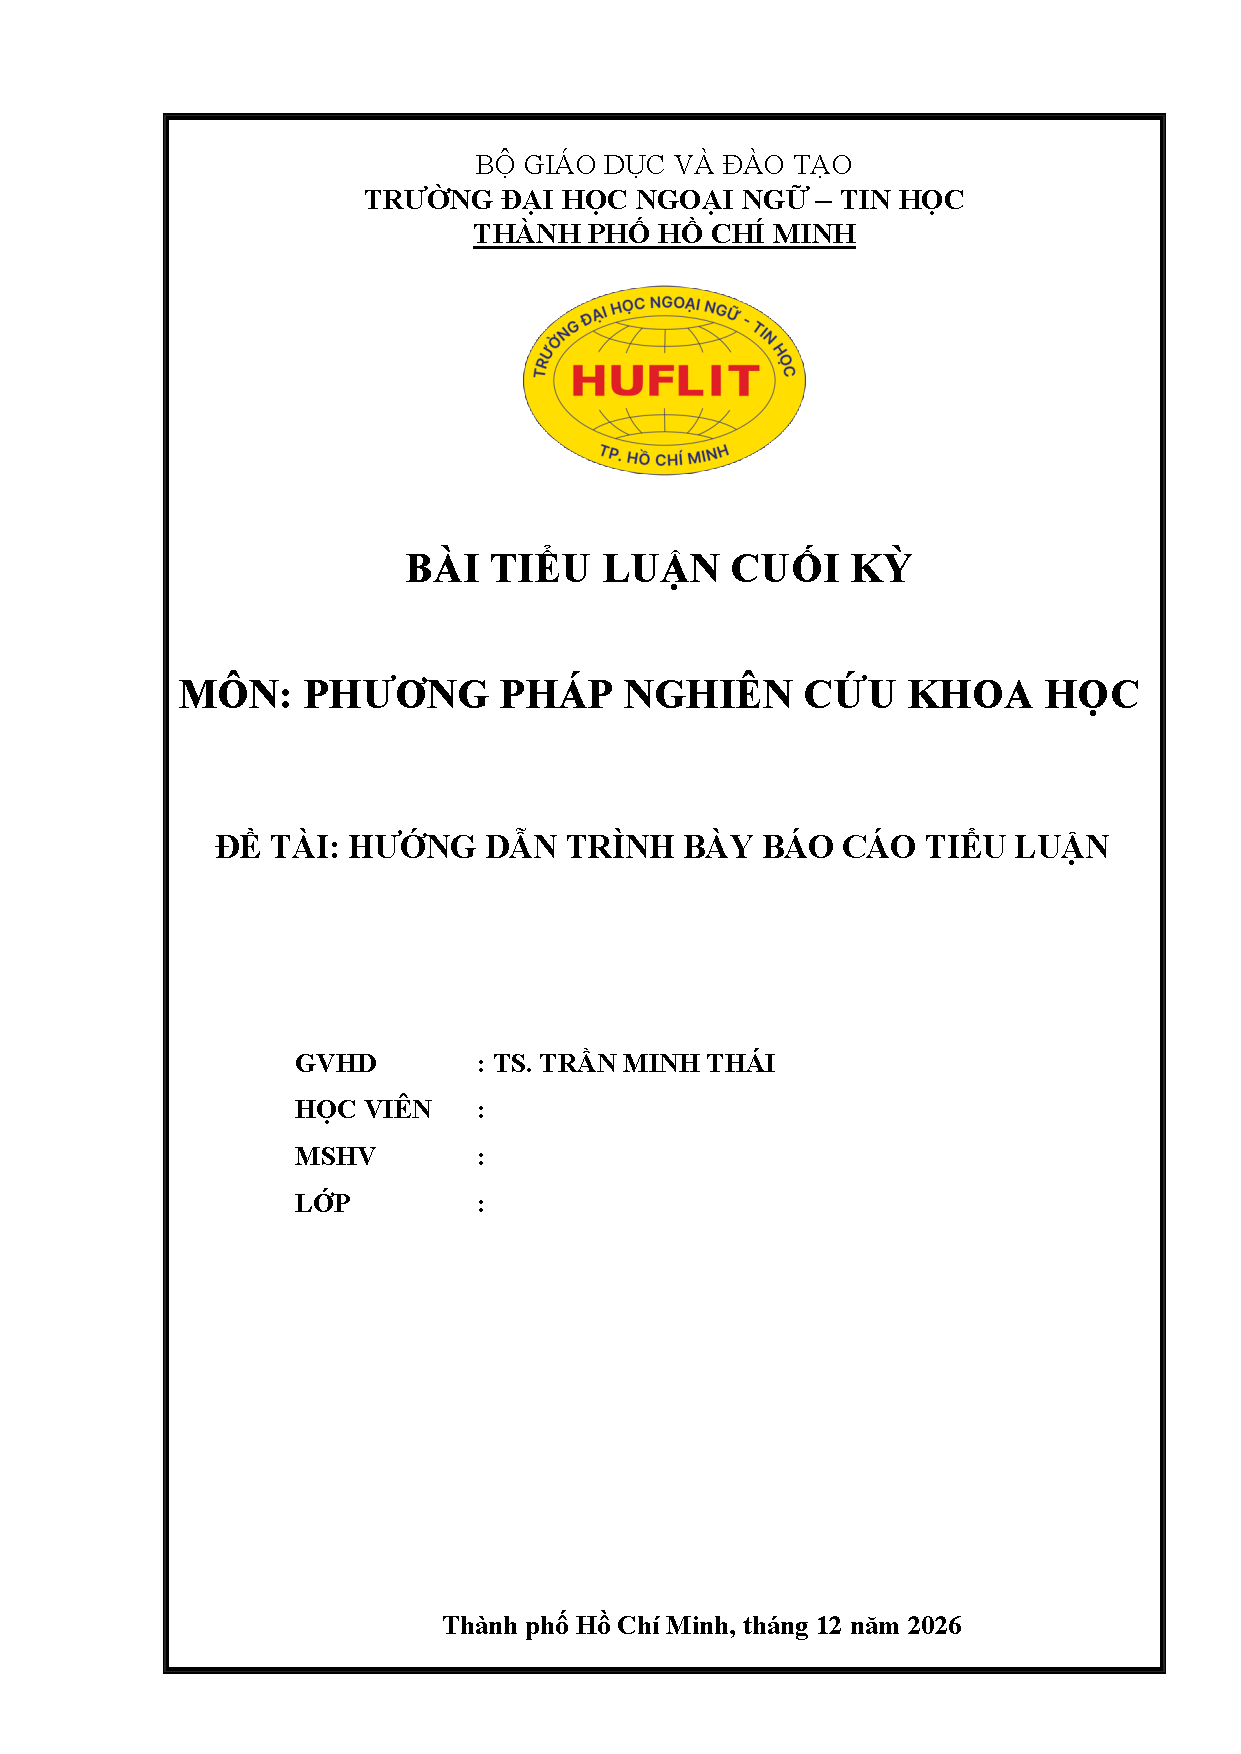
\includepdf[pages=-]{trangbia.pdf}

% --- II. CÁC PHẦN ĐẦU (Đánh số La-mã: i, ii, iii...) ---
% Trình tự: Nhận xét GV -> Lời cam đoan -> Lời cảm ơn -> Tóm tắt (bắt buộc)
% -> Danh mục từ viết tắt / bảng / hình -> Mục lục
\pagenumbering{roman}

% 1. Nhận xét của giảng viên hướng dẫn (để trống -- GV điền sau khi chấm)
% !TEX root = main.tex
% --- PHẦN NHẬN XÉT CỦA GIẢNG VIÊN ---
% Trang này ĐỂ TRỐNG để giảng viên viết tay nhận xét và điền điểm sau khi chấm
% (theo đúng bố cục trang "PHẦN NHẬN XÉT CỦA GIẢNG VIÊN" trong mẫu B20).
% Không đưa vào Mục lục vì đây là trang biểu mẫu hành chính, không phải nội dung
% do học viên biên soạn.

\chapter*{PHẦN NHẬN XÉT CỦA GIẢNG VIÊN}

% 5 dòng kẻ ngang để giảng viên viết tay nhận xét
\newcommand{\dongnhanxet}{\noindent\hspace*{1.27cm}\hrulefill\\[0.65cm]}
\vspace{0.3cm}
\dongnhanxet
\dongnhanxet
\dongnhanxet
\dongnhanxet
\dongnhanxet

\vspace{0.5cm}
% Khoanh oval trống để giảng viên viết điểm vào (đúng kích thước và vị trí như mẫu B20)
\noindent\hspace{1.27cm}\textbf{ĐIỂM:}\hspace{1cm}\raisebox{-0.55cm}{\tikz{\draw[thick] (0,0) ellipse (1.75cm and 0.95cm);}}

\vspace{0.3cm}
\noindent\hspace{2.54cm}Bằng chữ: \ldots\ldots\ldots\ldots\ldots\ldots\ldots\ldots

\vspace{1.2cm}
\begin{flushright}
\begin{minipage}{10.5cm}
\centering
\textit{Thành phố Hồ Chí Minh, ngày \ldots{} tháng \ldots{} năm 20\ldots}\\[0.5cm]
\textbf{Giảng viên chấm bài}\\[0.2cm]
\textit{(Ký tên và ghi rõ họ tên)}
\end{minipage}
\end{flushright}

\vspace{3cm}
\clearpage


% 2. Lời cam đoan (ký tên, ghi rõ ngày tháng)
% !TEX root = main.tex
% --- LỜI CAM ĐOAN ---
% Yêu cầu (Bài 05): ký tên, ghi rõ ngày tháng.
% Cam đoan về tính liêm chính học thuật: không đạo văn, trích dẫn đầy đủ theo IEEE.

\phantomsection
\addcontentsline{toc}{chapter}{LỜI CAM ĐOAN}
\chapter*{LỜI CAM ĐOAN}

\begin{spacing}{1.2}

Nội dung của phần này.

\end{spacing}

\vspace{1.5cm}
\begin{flushright}
\begin{minipage}{10.5cm}
\centering
Thành phố Hồ Chí Minh, ngày \ldots{} tháng \ldots{} năm 20\ldots\\[0.2cm]
\textbf{Học viên thực hiện}\\
\textit{(Ký tên và ghi rõ họ tên)}
\vspace{2.5cm}
\end{minipage}
\end{flushright}

\clearpage


% 3. Lời cảm ơn (ngắn gọn, không quá 1/2 trang)
% !TEX root = main.tex
% --- LỜI CẢM ƠN ---
% Yêu cầu (Bài 05): viết ngắn gọn, KHÔNG QUÁ 1/2 trang.

\phantomsection
\addcontentsline{toc}{chapter}{LỜI CẢM ƠN}
\chapter*{LỜI CẢM ƠN}

\begin{spacing}{1.2}

Nội dung của phần này.

\end{spacing}

\clearpage


% 4. Tóm tắt tiểu luận (BẮT BUỘC PHẢI CÓ)
% !TEX root = main.tex
% Tóm tắt tiểu luận -- trang bắt buộc, đặt sau Lời cảm ơn và trước các danh mục.

\phantomsection
\addcontentsline{toc}{chapter}{TÓM TẮT}
\chapter*{TÓM TẮT}

\begin{spacing}{1.2}

\begin{huongdan}
Tóm tắt khoảng 250--300 từ, trình bày thành một hoặc hai đoạn văn liền mạch (không gạch đầu dòng), khái quát toàn bộ đề cương theo bốn phần: (1) bối cảnh và vấn đề nghiên cứu (dựa trên Problem Statement ở mục~\ref{subsec:problem_statement}); (2) mục tiêu và câu hỏi nghiên cứu chính (mục~\ref{subsec:muc_tieu}, mục~\ref{subsec:rq}); (3) phương pháp và phạm vi dự kiến (mục~\ref{subsec:thiet_ke}); (4) kết quả và đóng góp dự kiến (mục~\ref{subsec:kq_ky_thuat}, mục~\ref{subsec:dong_gop_mo_rong}). Không dùng trích dẫn tài liệu tham khảo trong phần này.
\end{huongdan}

Nội dung của phần này.

\end{spacing}

\clearpage


% 5. Danh mục từ viết tắt
% !TEX root = main.tex
% --- DANH MỤC TỪ VIẾT TẮT (tự động tổng hợp) ---
% Bảng dưới đây được sinh tự động từ các lệnh \tvt{Viết tắt}{Ý nghĩa} đặt tại
% nơi từ viết tắt xuất hiện lần đầu trong Chương 1, 2, 3 (xem ví dụ DIKW, W5H2,
% FINER, MAPE, ROI, IEEE trong các chương). Bảng được tự động sắp xếp theo
% thứ tự ABC (tăng dần) của từ viết tắt. Học viên thêm \tvt cho từ viết tắt
% của riêng đề tài mình; KHÔNG cần gõ tay lại bảng này.

\phantomsection
\addcontentsline{toc}{chapter}{DANH MỤC TỪ VIẾT TẮT}
\chapter*{DANH MỤC TỪ VIẾT TẮT}

\dstuvt

\clearpage


% 6. Danh mục Bảng
\phantomsection
\addcontentsline{toc}{chapter}{DANH MỤC CÁC BẢNG}
\chapter*{DANH MỤC CÁC BẢNG}
\mhdanhmuc{lot}
\clearpage

% 7. Danh mục Hình vẽ, đồ thị
\phantomsection
\addcontentsline{toc}{chapter}{DANH MỤC CÁC HÌNH VẼ, ĐỒ THỊ}
\chapter*{DANH MỤC CÁC HÌNH VẼ, ĐỒ THỊ}
\mhdanhmuc{lof}
\clearpage

% 8. Mục lục
\phantomsection
\addcontentsline{toc}{chapter}{\textbf{MỤC LỤC}}
\tableofcontents
\clearpage

% --- III. NỘI DUNG CHÍNH: 3 CHƯƠNG + KẾT LUẬN (Đánh số Ả-rập: 1, 2, 3...) ---
\clearpage
\pagenumbering{arabic}

% !TEX root = main.tex
% Chương 1: Hệ thống hóa lý thuyết (20% tổng điểm, 4-6 trang)

\chapter{Hệ thống hóa lý thuyết}
\label{ch:chuong1}

\begin{spacing}{1.2}

\section*{Giới thiệu chương}

\begin{huongdan}
Trọng số: 20\% tổng điểm. Độ dài khuyến nghị: 5--10 trang. Chương này trình bày và phân tích các khái niệm nền tảng về phương pháp luận nghiên cứu khoa học đã học trong môn học. Không chép lại định nghĩa từ sách giáo khoa, mà tổng hợp, chắt lọc và kết nối lý thuyết với bối cảnh đề tài cụ thể của mình. Đoạn mở đầu này nên nêu ngắn gọn: chương gồm những mục nào (tương ứng Mục~\ref{sec:tri_thuc}, Mục~\ref{sec:quy_trinh_mo_hinh}, Mục~\ref{sec:dao_duc}) và mối liên hệ giữa chúng. Sau chương này cần đạt được: hệ thống hóa chu trình tri thức DIKW và ba phương pháp tư duy khoa học; mô tả và so sánh được ít nhất ba mô hình quy trình nghiên cứu; trình bày được các nguyên tắc đạo đức khoa học và cách áp dụng vào đề tài.
\end{huongdan}

Nội dung của phần này.

\section{Hệ thống tri thức khoa học (Knowledge System)}
\label{sec:tri_thuc}

\subsection{Chu trình DIKW -- từ dữ liệu đến lý thuyết}
\label{subsec:dikw}

\begin{huongdan}
Định nghĩa và mô tả bốn cấp độ: dữ liệu (Data), thông tin (Information), tri thức (Knowledge), lý thuyết/trí tuệ (Wisdom/Theory); mô tả quá trình chuyển đổi giữa các cấp; minh họa bằng ví dụ cụ thể từ lĩnh vực nghiên cứu của đề tài; nêu rõ đề tài đóng góp ở cấp độ nào trong chu trình DIKW.
\end{huongdan}

Nội dung của phần này. Chu trình \tvt{DIKW}{Data, Information, Knowledge, Wisdom -- các cấp độ của tri thức} là khung lý thuyết được sử dụng xuyên suốt mục này.

\subsection{Ba phương pháp tư duy khoa học}
\label{subsec:tu_duy}

\begin{huongdan}
Định nghĩa ngắn gọn từng phương pháp (diễn dịch, quy nạp, suy đoán), lấy ví dụ minh họa từ chính đề tài đang thực hiện, và chỉ rõ phương pháp nào là chủ đạo trong đề tài kèm lý do lựa chọn.
\end{huongdan}

Nội dung của phần này. Ba phương pháp tư duy khoa học được tóm tắt và liên hệ với đề tài tại Bảng~\ref{tab:tu_duy}.

\begin{table}[htpb]
\centering
\caption{So sánh ba phương pháp tư duy khoa học và ứng dụng trong đề tài}
\label{tab:tu_duy}
\renewcommand{\arraystretch}{1.3}
{\fontsize{12}{14}\selectfont
\begin{tabularx}{\textwidth}{|>{\raggedright\arraybackslash}p{3.2cm}|>{\raggedright\arraybackslash}p{4.6cm}|X|}
\hline
\textbf{Phương pháp} & \textbf{Hướng suy luận} & \textbf{Ứng dụng trong đề tài} \\
\hline
Diễn dịch (Deductive) & Lý thuyết chung $\rightarrow$ Trường hợp cụ thể & [Học viên điền ví dụ từ đề tài] \\
\hline
Quy nạp (Inductive) & Quan sát nhiều trường hợp $\rightarrow$ Quy luật chung & [Học viên điền ví dụ từ đề tài] \\
\hline
Suy đoán (Abductive) & Dữ kiện không đầy đủ $\rightarrow$ Giả thuyết tốt nhất & [Học viên điền ví dụ từ đề tài] \\
\hline
\end{tabularx}
}
\end{table}

\section{Quy trình và mô hình nghiên cứu}
\label{sec:quy_trinh_mo_hinh}

\subsection{Quy trình nghiên cứu khoa học cơ bản}
\label{subsec:quy_trinh}

\begin{huongdan}
Liệt kê và mô tả ít nhất bảy bước trong quy trình nghiên cứu khoa học cơ bản; giải thích mối liên hệ và phụ thuộc giữa các bước; chỉ ra bước dễ xảy ra sai lầm nhất và cách phòng tránh; ánh xạ từng bước vào kế hoạch thực hiện của đề tài.
\end{huongdan}

Nội dung của phần này. Quy trình nghiên cứu khoa học cơ bản gồm bảy bước, được trình bày một cách hệ thống trong giáo trình phương pháp luận nghiên cứu \cite{vidu_sach}, và được minh họa tại Hình~\ref{fig:quy_trinh_nc}.

\begin{figure}[htpb]
\centering
\begin{tikzpicture}[
  bstep/.style={rectangle, draw=blue!70, fill=blue!5, rounded corners,
               minimum width=7cm, minimum height=0.75cm, font=\small},
  arrow/.style={-{Stealth[scale=1.1]}, thick, draw=blue!80!black}
]
\node[bstep] (b1) {Bước 1: Xác định vấn đề};
\node[bstep, below=0.4cm of b1] (b2) {Bước 2: Tổng quan tài liệu};
\node[bstep, below=0.4cm of b2] (b3) {Bước 3: Xây dựng giả thuyết};
\node[bstep, below=0.4cm of b3] (b4) {Bước 4: Thiết kế nghiên cứu};
\node[bstep, below=0.4cm of b4] (b5) {Bước 5: Thu thập dữ liệu};
\node[bstep, below=0.4cm of b5] (b6) {Bước 6: Phân tích và diễn giải};
\node[bstep, below=0.4cm of b6] (b7) {Bước 7: Công bố và phản hồi};
\draw[arrow] (b1) -- (b2);
\draw[arrow] (b2) -- (b3);
\draw[arrow] (b3) -- (b4);
\draw[arrow] (b4) -- (b5);
\draw[arrow] (b5) -- (b6);
\draw[arrow] (b6) -- (b7);
\end{tikzpicture}
\caption{Quy trình nghiên cứu khoa học cơ bản (7 bước)}
\label{fig:quy_trinh_nc}
\end{figure}

\subsection{So sánh các mô hình nghiên cứu}
\label{subsec:so_sanh_mo_hinh}

\begin{huongdan}
Mô tả đặc điểm của ít nhất ba mô hình nghiên cứu: tuần tự (Sequential), vòng lặp (Iterative), tiến hóa (Evolutionary); phân tích ưu và nhược điểm của từng mô hình; lý giải cụ thể tại sao chọn một mô hình cho đề tài (không chỉ nói "phù hợp" mà không giải thích).
\end{huongdan}

Nội dung của phần này. Đặc điểm của ba mô hình nghiên cứu được so sánh tại Bảng~\ref{tab:mo_hinh_nc}.

\begin{table}[htpb]
\centering
\caption{So sánh các mô hình nghiên cứu}
\label{tab:mo_hinh_nc}
\renewcommand{\arraystretch}{1.3}
{\fontsize{12}{14}\selectfont
\begin{tabularx}{\textwidth}{|>{\raggedright\arraybackslash}p{2.8cm}|X|X|X|}
\hline
\textbf{Tiêu chí} & \textbf{Mô hình tuần tự} & \textbf{Mô hình vòng lặp} & \textbf{Mô hình tiến hóa} \\
\hline
Đặc điểm chính & Các bước thực hiện lần lượt, tuyến tính & Lặp lại các chu kỳ để cải tiến dần & Kết hợp nhiều phương pháp, thích nghi liên tục \\
\hline
Ưu điểm & Dễ quản lý, kế hoạch rõ ràng & Linh hoạt, phát hiện lỗi sớm & Thích hợp nghiên cứu phức tạp \\
\hline
Nhược điểm & Khó sửa đổi khi đã qua bước trước & Khó kiểm soát thời gian, phạm vi & Yêu cầu kinh nghiệm cao \\
\hline
Phù hợp khi & Bài toán rõ ràng, yêu cầu ổn định & Cần điều chỉnh dựa trên kết quả & Nghiên cứu dài hạn, phức tạp \\
\hline
Đề tài này dùng? & [Có / Không] & [Có / Không] & [Có / Không] \\
\hline
\end{tabularx}
}
\end{table}

\section{Đạo đức trong nghiên cứu khoa học}
\label{sec:dao_duc}

\subsection{Liêm chính học thuật và đạo văn (Plagiarism)}
\label{subsec:dao_van}

\begin{huongdan}
Định nghĩa đạo văn và các hình thức (sao chép nguyên văn, diễn giải không trích dẫn, tự đạo văn); trình bày kỹ thuật paraphrasing đúng cách kèm ví dụ câu gốc và câu diễn giải lại; nêu cách trích dẫn đúng theo chuẩn IEEE; kết thúc bằng cam kết của học viên về tính liêm chính trong tiểu luận này.
\end{huongdan}

Nội dung của phần này. Chuẩn trích dẫn \tvt{IEEE}{Institute of Electrical and Electronics Engineers} được áp dụng thống nhất cho toàn bộ tiểu luận.

\subsection{Đạo đức thu thập và sử dụng dữ liệu}
\label{subsec:dao_duc_du_lieu}

\begin{huongdan}
Trình bày nguyên tắc bảo mật dữ liệu doanh nghiệp (xin phép, ký thỏa thuận bảo mật, ẩn danh hóa); quyền riêng tư của người dùng/khách hàng trong dữ liệu thu thập; trách nhiệm công bố kết quả trung thực; kết thúc bằng cam kết cụ thể về cách đảm bảo đạo đức trong đề tài.
\end{huongdan}

Nội dung của phần này.

\section{Tổng kết chương 1}
\label{sec:tong_ket_c1}

\begin{huongdan}
Điểm lại ngắn gọn ba nội dung chính đã trình bày: chu trình DIKW và các phương pháp tư duy khoa học (Mục~\ref{sec:tri_thuc}); quy trình và mô hình nghiên cứu đã chọn (Mục~\ref{sec:quy_trinh_mo_hinh}); các nguyên tắc đạo đức khoa học sẽ tuân thủ (Mục~\ref{sec:dao_duc}). Kết thúc bằng một câu chuyển ý sang Chương 2, ví dụ: khung lý thuyết vừa hệ thống hóa sẽ được vận dụng để phân tích bài toán thực tế tại doanh nghiệp.
\end{huongdan}

Nội dung của phần này.

\end{spacing}
   % Chương 1: Hệ thống hóa lý thuyết (20%, 4-6 trang)
% !TEX root = main.tex
% Chương 2: Xác lập nền tảng và ứng dụng công cụ (30% tổng điểm, 6-9 trang)

\chapter{Xác lập nền tảng và ứng dụng công cụ}
\label{ch:chuong2}

\begin{spacing}{1.2}

\section*{Giới thiệu chương}

\begin{huongdan}
Trọng số: 30\% tổng điểm. Độ dài khuyến nghị: 10--15 trang. Chương này nặng về bằng chứng thực tế. Mỗi luận điểm cần minh chứng bằng số liệu cụ thể từ doanh nghiệp hoặc trích dẫn từ bài báo khoa học, tránh viết chung chung. Đoạn mở đầu này nên nêu ngắn gọn chương gồm những mục nào (Mục~\ref{sec:bai_toan_dn}, Mục~\ref{sec:cong_cu_tai_lieu}, Mục~\ref{sec:synthesis}) và cách chúng nối tiếp nhau. Sau chương này cần đạt được: phân tích được bài toán doanh nghiệp theo khung W5H2 với số liệu cụ thể; có minh chứng (ảnh chụp màn hình) việc sử dụng Mendeley/Zotero cho ít nhất năm bài báo; thiết lập bộ tiêu chí đánh giá độ tin cậy nguồn tài liệu (theo nguyên tắc Think-Check-Submit, loại trừ xuất bản săn mồi/trục lợi) và minh chứng tra cứu xếp hạng học thuật (SCImago SJR Q1/Q2 cho tạp chí, CORE Ranking A*/A/B cho hội nghị); lập được ma trận tổng hợp và viết đoạn phân tích Research Gap rõ ràng.
\end{huongdan}

Nội dung của phần này.

\section{Phân tích bài toán tại doanh nghiệp}
\label{sec:bai_toan_dn}

\subsection{Tổng quan doanh nghiệp khảo sát}
\label{subsec:tong_quan_dn}

\begin{huongdan}
Nêu tên/loại hình doanh nghiệp (dùng tên giả nếu cần bảo mật), quy mô, lĩnh vực hoạt động, hạ tầng CNTT hiện tại, mức độ trưởng thành số hóa. Sau bảng, viết một đoạn văn tóm tắt khoảng 100 từ kết nối các thông tin, không liệt kê đơn thuần.
\end{huongdan}

Nội dung của phần này. Thông tin tổng quan về doanh nghiệp khảo sát được trình bày tại Bảng~\ref{tab:thong_tin_dn}.

\begin{table}[htpb]
\centering
\caption{Thông tin doanh nghiệp khảo sát}
\label{tab:thong_tin_dn}
\renewcommand{\arraystretch}{1.3}
{\fontsize{12}{14}\selectfont
\begin{tabularx}{\textwidth}{|>{\raggedright\arraybackslash}p{5cm}|X|}
\hline
\textbf{Tiêu chí} & \textbf{Thông tin doanh nghiệp (Học viên điền)} \\
\hline
Tên doanh nghiệp & [Tên chính thức hoặc tên giả nếu bảo mật] \\
\hline
Lĩnh vực hoạt động & [Bán lẻ / Sản xuất / Logistics / FinTech\ldots] \\
\hline
Quy mô nhân sự, chi nhánh & [X nhân viên, X chi nhánh tại\ldots] \\
\hline
Hạ tầng CNTT (phần cứng, phần mềm) & [On-premise / Cloud; ERP, CRM\ldots] \\
\hline
Loại và khối lượng dữ liệu & [Giao dịch POS / Khách hàng; $\sim$X GB/năm] \\
\hline
Mức độ số hóa hiện tại & [Mới bắt đầu / Đang triển khai / Đã hoàn thiện] \\
\hline
\end{tabularx}
}
\end{table}

\subsection{Xác định vấn đề theo khung W5H2}
\label{subsec:w5h2}

\begin{huongdan}
Trả lời đầy đủ sáu chiều phân tích, mỗi chiều ít nhất hai đến ba câu, có số liệu định lượng cụ thể (thiệt hại, tỷ lệ phần trăm, thời gian, chi phí); xác định nguyên nhân gốc rễ, không chỉ mô tả triệu chứng.
\end{huongdan}

Nội dung của phần này. Kết quả phân tích vấn đề theo khung \tvt{W5H2}{What, Who, Where, When, Why, How much -- sáu chiều phân tích vấn đề} được tổng hợp tại Bảng~\ref{tab:w5h2}.

\begin{table}[htpb]
\centering
\caption{Phân tích vấn đề theo khung W5H2}
\label{tab:w5h2}
\renewcommand{\arraystretch}{1.3}
{\fontsize{12}{14}\selectfont
\begin{tabularx}{\textwidth}{|>{\raggedright\arraybackslash}p{2.6cm}|>{\raggedright\arraybackslash}p{4.6cm}|X|}
\hline
\textbf{Chiều} & \textbf{Câu hỏi} & \textbf{Phân tích chi tiết (cần có số liệu)} \\
\hline
WHAT? & Bài toán/thách thức cụ thể là gì? & [Học viên điền] \\
\hline
WHO? & Bộ phận/người nào bị ảnh hưởng? & [Học viên điền] \\
\hline
WHERE? & Vấn đề xảy ra tại đâu? & [Học viên điền] \\
\hline
WHEN? & Tần suất và thời điểm xảy ra? & [Học viên điền] \\
\hline
WHY? & Nguyên nhân gốc rễ là gì? & [Học viên điền] \\
\hline
HOW MUCH? & Chi phí/tổn thất cụ thể là bao nhiêu? & [Học viên điền] \\
\hline
\end{tabularx}
}
\end{table}

\subsection{Phát biểu vấn đề nghiên cứu (Problem Statement)}
\label{subsec:problem_statement}

\begin{huongdan}
Viết một đoạn văn súc tích, đo lường được, tổng hợp từ kết quả phân tích W5H2, theo cấu trúc: [Tên doanh nghiệp], một [loại hình] với [quy mô], đang đối mặt với vấn đề [mô tả cụ thể], dẫn đến [hậu quả đo lường được]. Mặc dù [giải pháp hiện tại], hiệu quả chỉ đạt [con số]. Khoảng trống: chưa có [điều gì] để [mục tiêu]. Nghiên cứu này đề xuất [giải pháp] nhằm đạt [kết quả kỳ vọng] trong [thời gian].
\end{huongdan}

Nội dung của phần này.

\section{Ứng dụng công cụ quản lý tài liệu (Mendeley/Zotero)}
\label{sec:cong_cu_tai_lieu}

\subsection{Giới thiệu công cụ và lý do lựa chọn}
\label{subsec:gioi_thieu_cong_cu}

\begin{huongdan}
Giới thiệu ngắn gọn Mendeley và Zotero, nêu lý do chọn công cụ cụ thể cho tiểu luận này, và mô tả quy trình làm việc khoa học: tìm kiếm bài báo từ các cơ sở dữ liệu uy tín (Scopus, Web of Science, IEEE Xplore), nhập vào thư viện, thẩm định độ tin cậy và xếp hạng, gắn thẻ phân loại (theo chủ đề, phân vị Q1/Q2 hoặc CORE A*/A), và trích xuất trích dẫn theo định dạng IEEE.
\end{huongdan}

Nội dung của phần này.

\subsection{Minh chứng sử dụng công cụ (ảnh màn hình)}
\label{subsec:minh_chung_cong_cu}

\begin{huongdan}
Cần đủ bốn ảnh màn hình: (1) thư viện hiển thị ít nhất năm bài báo với metadata đầy đủ; (2) gắn thẻ phân loại bài báo theo chủ đề và xếp hạng học thuật (ví dụ: gắn thẻ Q1, Q2, CORE A, Scopus để phục vụ quản lý và sàng lọc); (3) chi tiết metadata của một bài báo (DOI, tóm tắt, nguồn, ấn phẩm); (4) thao tác xuất trích dẫn theo định dạng IEEE. Mỗi hình phải có chú thích và được tham chiếu trong văn bản; sau mỗi hình viết thêm hai đến ba câu mô tả ý nghĩa.
\end{huongdan}

Nội dung của phần này. Hình~\ref{fig:mendeley} minh họa thư viện tài liệu được xây dựng cho đề tài.

\begin{figure}[htpb]
\centering
\begin{tikzpicture}
\draw[dashed, thick, gray, rounded corners] (0,0) rectangle (13.5,5.5);
\node[align=center, gray, font=\small] at (6.75,2.75)
  {[Chèn ảnh chụp màn hình thư viện Mendeley/Zotero\\
   hiển thị tối thiểu 5 bài báo với metadata đầy đủ và gắn thẻ xếp hạng (Q1/Q2/CORE)]\\[0.5em]
   (Cần đủ 4 hình: thư viện, gắn thẻ phân loại chủ đề \& xếp hạng, chi tiết bài báo, xuất trích dẫn IEEE)};
\end{tikzpicture}
\caption{Thư viện Mendeley/Zotero với 5 bài báo liên quan đến đề tài}
\label{fig:mendeley}
\end{figure}

\section{Ma trận tổng hợp tài liệu (Synthesis Matrix)}
\label{sec:synthesis}

\subsection{Tiêu chí chọn lọc và đánh giá độ tin cậy, xếp hạng bài báo}
\label{subsec:tieu_chi_chon_bai}

\begin{huongdan}
Chọn năm bài báo xuất bản trong năm năm gần nhất, từ nguồn học thuật uy tín và cơ sở dữ liệu hàng đầu (IEEE Xplore, ACM Digital Library, SpringerLink, Elsevier ScienceDirect, Scopus, Web of Science). Trình bày rõ các tiêu chí lựa chọn và loại trừ (Inclusion/Exclusion Criteria) bao gồm: tính thời sự (trong vòng 5 năm gần nhất), độ liên quan trực tiếp đến bài toán nghiên cứu, phương pháp luận chặt chẽ, và đặc biệt là độ tin cậy của ấn phẩm (quy chuẩn Think-Check-Submit, loại trừ tuyệt đối tạp chí săn mồi/kém chất lượng) cùng chuẩn xếp hạng học thuật bắt buộc (tạp chí đạt phân vị SCImago SJR Q1/Q2; hội nghị đạt chuẩn CORE Ranking A*/A/B). Mô tả chiến lược tìm kiếm: từ khóa sử dụng (kết hợp toán tử Boolean AND/OR), cơ sở dữ liệu tra cứu, số lượng kết quả thu được ở từng bước và lý do tinh lọc ra năm bài báo này.
\end{huongdan}

Nội dung của phần này. Chiến lược tìm kiếm và tiêu chí chọn lọc bài báo được xây dựng nhằm bảo đảm tính cập nhật, độ tin cậy học thuật và chất lượng nghiên cứu cao nhất. Các tài liệu được sàng lọc qua cơ sở dữ liệu Scopus, Web of Science và IEEE Xplore, tuân thủ nghiêm ngặt bộ tiêu chí an toàn xuất bản Think-Check-Submit và đối chiếu hệ thống xếp hạng SCImago Journal Rank (SJR) cùng CORE Conference Ranking. Kết quả đánh giá độ tin cậy và xếp hạng của 5 bài báo tiêu biểu được tổng hợp tại Bảng~\ref{tab:danh_gia_xep_hang}. Minh chứng tra cứu xếp hạng trực tuyến từ cổng SCImago và CORE Portal được thể hiện tại Hình~\ref{fig:minh_chung_xep_hang}.

% BẢNG ĐÁNH GIÁ ĐỘ TIN CẬY VÀ XẾP HẠNG TÀI LIỆU
\begin{table}[htpb]
\centering
\caption{Đánh giá độ tin cậy và xếp hạng của các tài liệu nghiên cứu}
\label{tab:danh_gia_xep_hang}
\renewcommand{\arraystretch}{1.3}
{\fontsize{10}{12}\selectfont
\begin{tabularx}{\textwidth}{|>{\centering\arraybackslash}p{1.4cm}|>{\raggedright\arraybackslash}X|>{\centering\arraybackslash}p{2.3cm}|>{\centering\arraybackslash}p{2.6cm}|>{\raggedright\arraybackslash}X|}
\hline
\textbf{Bài báo} & \textbf{Tên ấn phẩm \& NXB} & \textbf{CSDL chỉ mục} & \textbf{Xếp hạng (SJR / CORE)} & \textbf{Thẩm định độ tin cậy (Think-Check-Submit)} \\
\hline
\cite{vidu_tapchi} & IEEE Transactions on Software Engineering (IEEE) & Scopus, WoS (SCIE) & SJR Q1 (IF: 6.5, CiteScore: 12.8) & Tạp chí đầu ngành, quy trình bình duyệt ngang hàng nghiêm ngặt; không nằm trong danh mục cảnh báo/săn mồi. \\
\hline
\cite{vidu_hoinghi} & International Conference on Software Engineering (ACM/IEEE) & Scopus, WoS, DBLP & CORE Rank A* (Flagship) & Hội thảo khoa học máy tính hàng đầu; tỷ lệ chấp nhận bài $\sim$18\%; ban chương trình quốc tế uy tín. \\
\hline
[Bài báo 3] & [Điền tên Tạp chí/Hội thảo, NXB] & [Scopus / WoS] & [SJR Q1/Q2 / CORE A*/A/B] & [Điền kết quả kiểm tra Think-Check-Submit: phản biện minh bạch, NXB uy tín, chỉ mục chuẩn] \\
\hline
[Bài báo 4] & [Điền tên Tạp chí/Hội thảo, NXB] & [Scopus / WoS] & [SJR Q1/Q2 / CORE A*/A/B] & [Điền kết quả kiểm tra Think-Check-Submit: phản biện minh bạch, NXB uy tín, chỉ mục chuẩn] \\
\hline
[Bài báo 5] & [Điền tên Tạp chí/Hội thảo, NXB] & [Scopus / WoS] & [SJR Q1/Q2 / CORE A*/A/B] & [Điền kết quả kiểm tra Think-Check-Submit: phản biện minh bạch, NXB uy tín, chỉ mục chuẩn] \\
\hline
\end{tabularx}
}
\end{table}

% HÌNH MINH CHỨNG TRA CỨU XẾP HẠNG VÀ ĐỘ TIN CẬY
\begin{figure}[htpb]
\centering
\begin{tikzpicture}
\draw[dashed, thick, gray, rounded corners] (0,0) rectangle (13.5,6.0);
\node[align=center, gray, font=\small] at (6.75,3.0)
  {\textbf{[Chèn ảnh chụp màn hình minh chứng tra cứu xếp hạng và độ tin cậy của tài liệu]}\\[0.6em]
   \textit{(Cần tối thiểu 2--3 ảnh màn hình tra cứu từ các nguồn cơ sở dữ liệu chính thống):}\\[0.5em]
   \textbf{1. Minh chứng SCImago Journal Rank (SJR):} Tra cứu tại \texttt{scimagojr.com},\\
   thể hiện rõ tên tạp chí, phân hạng Quartile (Q1/Q2), chỉ số SJR và CSDL Scopus;\\[0.3em]
   \textbf{2. Minh chứng CORE Conference Ranking:} Tra cứu tại \texttt{portal.core.edu.au},\\
   thể hiện tên hội thảo khoa học máy tính, niên khóa và xếp hạng (Rank A*, A, hoặc B);\\[0.3em]
   \textbf{3. Minh chứng chỉ mục CSDL \& An toàn xuất bản:} Tra cứu trên Scopus/WoS Master Journal List\\
   hoặc quy chuẩn Think-Check-Submit nhằm chứng minh không thuộc ấn phẩm săn mồi/trục lợi.};
\end{tikzpicture}
\caption{Minh chứng tra cứu xếp hạng SCImago/CORE và thẩm định nguồn tài liệu tin cậy}
\label{fig:minh_chung_xep_hang}
\end{figure}

\subsection{Ma trận tổng hợp 5 bài báo}
\label{subsec:ma_tran}

\begin{huongdan}
So sánh năm bài báo theo các tiêu chí: trích dẫn IEEE đầy đủ kèm phân hạng học thuật (SJR Q1/Q2 hoặc CORE A*/A), vấn đề nghiên cứu chính, phương pháp, dữ liệu và quy mô, chỉ số đánh giá, kết quả nổi bật, điểm mạnh, hạn chế (GAP), bối cảnh địa lý và mức độ liên quan.
\end{huongdan}

Nội dung của phần này. Kết quả tổng hợp và so sánh các nghiên cứu liên quan được trình bày tại Bảng~\ref{tab:synthesis_matrix}. Hai dòng đầu minh họa cách trích dẫn thực tế bằng lệnh \texttt{\textbackslash cite} kết hợp thông tin phân hạng học thuật, giúp số thứ tự bài báo và Tài liệu tham khảo tự động khớp nhau; ba dòng còn lại là chỗ trống để học viên điền bài báo của đề tài mình.

\begin{table}[htpb]
\centering
\caption{Ma trận tổng hợp các nghiên cứu liên quan}
\label{tab:synthesis_matrix}
\renewcommand{\arraystretch}{1.3}
{\fontsize{10}{12}\selectfont
\begin{tabularx}{\textwidth}{|>{\centering\arraybackslash}p{1.8cm}|X|X|X|X|X|}
\hline
\textbf{Bài báo \& Xếp hạng} & \textbf{Vấn đề nghiên cứu} & \textbf{Phương pháp} & \textbf{Dữ liệu} & \textbf{Kết quả nổi bật} & \textbf{Hạn chế (GAP)} \\
\hline
\cite{vidu_tapchi}\newline \textbf{(SJR Q1)} & [Điền] & [Điền] & [Điền] & [Điền] & [Điền] \\
\hline
\cite{vidu_hoinghi}\newline \textbf{(CORE A*)} & [Điền] & [Điền] & [Điền] & [Điền] & [Điền] \\
\hline
[Bài báo 3]\newline \textbf{([Q1/Q2/A])} & [Điền] & [Điền] & [Điền] & [Điền] & [Điền] \\
\hline
[Bài báo 4]\newline \textbf{([Q1/Q2/A])} & [Điền] & [Điền] & [Điền] & [Điền] & [Điền] \\
\hline
[Bài báo 5]\newline \textbf{([Q1/Q2/A])} & [Điền] & [Điền] & [Điền] & [Điền] & [Điền] \\
\hline
\end{tabularx}
}
\end{table}

\subsection{Phân tích khoảng trống nghiên cứu (Research Gap)}
\label{subsec:research_gap}

\begin{huongdan}
Đây là mục quan trọng nhất của chương. Viết đoạn phân tích tổng hợp tối thiểu 200 từ, gồm: xu hướng chung mà các nghiên cứu đã đồng thuận (hai đến ba điểm); hạn chế còn tồn tại mà chưa nghiên cứu nào giải quyết; Research Gap cụ thể, đặc biệt trong bối cảnh Việt Nam hoặc đặc thù đề tài; và phần kết nối giải thích tại sao khoảng trống này đặt ra sự cần thiết cho nghiên cứu của bạn.
\end{huongdan}

Nội dung của phần này.

\section{Tổng kết chương 2}
\label{sec:tong_ket_c2}

\begin{huongdan}
Điểm lại ngắn gọn: bài toán doanh nghiệp đã phân tích theo khung W5H2 và Problem Statement (Mục~\ref{sec:bai_toan_dn}); quy trình ứng dụng công cụ quản lý tài liệu và thẩm định độ tin cậy, xếp hạng học thuật (Mục~\ref{sec:cong_cu_tai_lieu} và Mục~\ref{sec:synthesis}); và khoảng trống nghiên cứu đã xác định qua ma trận tổng hợp (Mục~\ref{sec:synthesis}). Kết thúc bằng câu chuyển ý sang Chương 3, ví dụ: khoảng trống nghiên cứu vừa xác định trên nền tảng các tài liệu khoa học uy tín sẽ là cơ sở vững chắc để xây dựng đề cương nghiên cứu chi tiết.
\end{huongdan}

Nội dung của phần này.

\end{spacing}
   % Chương 2: Xác lập nền tảng và ứng dụng công cụ (30%, 6-9 trang)
% !TEX root = main.tex
% Chương 3: Xây dựng đề cương nghiên cứu chi tiết (45% tổng điểm, 9-14 trang)
% Lưu ý kỹ thuật: mọi bảng/hình/công thức PHẢI được tham chiếu trong văn bản
% bằng \ref{...} -- không để bảng/hình/công thức "mồ côi".

\chapter{Xây dựng đề cương nghiên cứu chi tiết}
\label{ch:chuong3}

\begin{spacing}{1.2}

\section*{Giới thiệu chương}

\begin{huongdan}
Trọng số: 45\% tổng điểm, chương trọng tâm nhất của tiểu luận. Độ dài khuyến nghị: 10--15 trang. Thiết kế một đề cương nghiên cứu thực sự khả thi, đủ chi tiết để người đọc hình dung rõ cách thực hiện, đánh giá và triển khai đề tài. Mọi khẳng định phải được hỗ trợ bởi bằng chứng khoa học (trích dẫn từ Chương 2) hoặc số liệu thực tế từ doanh nghiệp, vì đây là nơi Chương 1, 2 và 3 phải liên kết chặt chẽ với nhau. Đoạn mở đầu này nên nêu ngắn gọn chương gồm những mục nào (Mục~\ref{sec:tieu_de_muc_tieu} đến Mục~\ref{sec:ket_qua_du_kien}) và mạch triển khai giữa chúng. Sau chương này cần đạt được: xây dựng tiêu đề chuẩn và các mục tiêu nghiên cứu đo lường được; kiểm tra tính khả thi qua khung FINER với bằng chứng cụ thể; thiết kế phương pháp nghiên cứu đủ chi tiết để triển khai thực tế; lập kế hoạch thực hiện, quản lý rủi ro và dự kiến kết quả đầu ra.
\end{huongdan}

Nội dung của phần này.

\section{Tiêu đề và mục tiêu nghiên cứu}
\label{sec:tieu_de_muc_tieu}

\subsection{Xây dựng tiêu đề nghiên cứu}
\label{subsec:tieu_de}

\begin{huongdan}
Một tiêu đề tốt phải trả lời được ba câu hỏi: phương pháp/công nghệ gì, để làm gì, cho ai/ở đâu. Trình bày tiêu đề chính thức; phân tích từng thành phần của tiêu đề; giải thích tiêu đề phản ánh đúng Research Gap đã xác định ở Chương 2 như thế nào; nêu ít nhất một tiêu đề thay thế đã cân nhắc và lý do không chọn.
\end{huongdan}

Nội dung của phần này.

\subsection{Mục tiêu nghiên cứu}
\label{subsec:muc_tieu}

\begin{huongdan}
Mục tiêu tổng quát (GO) trình bày trong một đến hai câu, bắt đầu bằng động từ hành động. Mục tiêu cụ thể (SO1, SO2...) gồm ba đến năm mục tiêu nhỏ, mỗi mục cụ thể, đo lường được và đóng góp trực tiếp cho mục tiêu tổng quát.
\end{huongdan}

Nội dung của phần này. Hệ thống mục tiêu nghiên cứu được trình bày tại Bảng~\ref{tab:muc_tieu}.

\begin{table}[htpb]
\centering
\caption{Mục tiêu nghiên cứu tổng quát và cụ thể}
\label{tab:muc_tieu}
\renewcommand{\arraystretch}{1.3}
{\fontsize{12}{14}\selectfont
\begin{tabularx}{\textwidth}{|>{\raggedright\arraybackslash}p{2.6cm}|X|>{\raggedright\arraybackslash}p{4cm}|}
\hline
\textbf{Mục tiêu} & \textbf{Nội dung} & \textbf{Chỉ số đo lường} \\
\hline
GO (tổng quát) & [Học viên điền] & N/A -- bao quát \\
\hline
SO1 & [Học viên điền] & [Chỉ số cụ thể] \\
\hline
SO2 & [Học viên điền] & [Chỉ số cụ thể] \\
\hline
SO3 & [Học viên điền] & [Chỉ số cụ thể] \\
\hline
\end{tabularx}
}
\end{table}

\section{Câu hỏi nghiên cứu và kiểm tra FINER}
\label{sec:rq_finer}

\subsection{Câu hỏi nghiên cứu (Research Questions)}
\label{subsec:rq}

\begin{huongdan}
Nêu một câu hỏi nghiên cứu chính (MRQ) bao quát toàn bộ đề tài, và ba đến năm câu hỏi phụ (RQ1, RQ2...) cụ thể, mỗi câu trả lời được bằng dữ liệu thu thập được. Lập bảng liên kết mỗi câu hỏi với phương pháp và kết quả tương ứng.
\end{huongdan}

Nội dung của phần này. Hệ thống câu hỏi nghiên cứu được tổng hợp tại Bảng~\ref{tab:rq}.

\begin{table}[htpb]
\centering
\caption{Câu hỏi nghiên cứu và phương pháp trả lời}
\label{tab:rq}
\renewcommand{\arraystretch}{1.3}
{\fontsize{12}{14}\selectfont
\begin{tabularx}{\textwidth}{|>{\raggedright\arraybackslash}p{1.8cm}|X|>{\raggedright\arraybackslash}p{3.6cm}|>{\raggedright\arraybackslash}p{3.2cm}|}
\hline
\textbf{Câu hỏi} & \textbf{Nội dung} & \textbf{Phương pháp trả lời} & \textbf{Kết quả kỳ vọng} \\
\hline
MRQ & [Học viên điền] & Toàn bộ quy trình & [Điền] \\
\hline
RQ1 & [Học viên điền] & [Điền] & [Điền] \\
\hline
RQ2 & [Học viên điền] & [Điền] & [Điền] \\
\hline
RQ3 & [Học viên điền] & [Điền] & [Điền] \\
\hline
\end{tabularx}
}
\end{table}

\subsection{Kiểm tra tiêu chí FINER}
\label{subsec:finer}

\begin{huongdan}
Trả lời từng tiêu chí (Feasible, Interesting, Novel, Ethical, Relevant) bằng bằng chứng cụ thể, không chỉ ghi "Có" hay "Đạt". Tiêu chí Novel phải liên kết với Research Gap ở mục~\ref{subsec:research_gap}; tiêu chí Relevant phải liên kết với Problem Statement ở mục~\ref{subsec:problem_statement}.
\end{huongdan}

Nội dung của phần này. Kết quả kiểm tra tính khả thi của đề tài theo khung \tvt{FINER}{Feasible, Interesting, Novel, Ethical, Relevant} được trình bày tại Bảng~\ref{tab:finer}.

\begin{table}[htpb]
\centering
\caption{Kiểm tra đề tài theo khung FINER}
\label{tab:finer}
\renewcommand{\arraystretch}{1.3}
{\fontsize{12}{14}\selectfont
\begin{tabularx}{\textwidth}{|>{\raggedright\arraybackslash}p{3.4cm}|>{\raggedright\arraybackslash}p{5.2cm}|X|}
\hline
\textbf{Tiêu chí} & \textbf{Câu hỏi đánh giá} & \textbf{Bằng chứng cụ thể} \\
\hline
F -- Feasible (Khả thi) & Có đủ dữ liệu, kỹ năng, ngân sách, thời gian? & [Học viên điền] \\
\hline
I -- Interesting (Thú vị) & Kết quả có ý nghĩa với khoa học và xã hội? & [Học viên điền] \\
\hline
N -- Novel (Mới mẻ) & Có gì khác so với nghiên cứu đã có? & [Liên kết Research Gap, mục~\ref{subsec:research_gap}] \\
\hline
E -- Ethical (Đạo đức) & Dữ liệu hợp pháp? Quyền riêng tư? & [Học viên điền] \\
\hline
R -- Relevant (Liên quan) & Giải quyết vấn đề thực tiễn cấp thiết? & [Liên kết Problem Statement, mục~\ref{subsec:problem_statement}] \\
\hline
\end{tabularx}
}
\end{table}

\section{Phương pháp nghiên cứu dự kiến}
\label{sec:phuong_phap_nc}

\subsection{Loại hình nghiên cứu và thiết kế tổng thể}
\label{subsec:thiet_ke}

\begin{huongdan}
Xác định loại hình nghiên cứu (thực nghiệm, khảo sát, case study, hay kết hợp) kèm lý do chọn; mô tả thiết kế nghiên cứu tổng thể bằng sơ đồ luồng; xác định biến độc lập, biến phụ thuộc, biến kiểm soát; nêu phương pháp đánh giá, kiểm chứng và cơ sở so sánh (baseline).
\end{huongdan}

Nội dung của phần này. Thiết kế nghiên cứu tổng thể được minh họa tại Hình~\ref{fig:thiet_ke_nc}.

\begin{figure}[htpb]
\centering
\begin{tikzpicture}[
  block/.style={rectangle, draw=green!60!black, fill=green!5, rounded corners,
                minimum height=1.1cm, text width=2.3cm, align=center, font=\small},
  arrow/.style={-{Stealth[scale=1.1]}, thick, draw=green!50!black}
]
\node[block] (b1) {Thu thập dữ liệu};
\node[block, right=0.55cm of b1] (b2) {Tiền xử lý};
\node[block, right=0.55cm of b2] (b3) {Xây dựng giải pháp};
\node[block, right=0.55cm of b3] (b4) {Đánh giá};
\node[block, right=0.55cm of b4] (b5) {Triển khai};
\draw[arrow] (b1) -- (b2);
\draw[arrow] (b2) -- (b3);
\draw[arrow] (b3) -- (b4);
\draw[arrow] (b4) -- (b5);
\end{tikzpicture}
\caption{Sơ đồ thiết kế nghiên cứu tổng thể (học viên điều chỉnh theo đề tài)}
\label{fig:thiet_ke_nc}
\end{figure}

\subsection{Quy trình thu thập dữ liệu}
\label{subsec:thu_thap_du_lieu}

\begin{huongdan}
Nêu nguồn dữ liệu (hệ thống, loại, định dạng, thời gian); phương pháp thu thập (truy vấn SQL, gọi API, xuất tệp, khảo sát...); quy mô dữ liệu dự kiến; quy trình làm sạch, chuẩn hóa, tạo đặc trưng; và kế hoạch xử lý khi gặp vấn đề dữ liệu.
\end{huongdan}

Nội dung của phần này.

\subsection{Phương pháp phân tích và công nghệ sử dụng}
\label{subsec:phan_tich_cong_nghe}

\begin{huongdan}
Mô tả thuật toán/mô hình sẽ áp dụng (nguyên lý hoạt động, tham số chính, lý do phù hợp); liệt kê đầy đủ công nghệ sử dụng (ngôn ngữ lập trình, thư viện, framework, cơ sở dữ liệu, nền tảng đám mây, công cụ trực quan hóa); nêu quy trình huấn luyện/thực hiện và kiến trúc hệ thống.
\end{huongdan}

Để minh họa cách trình bày một độ đo định lượng có công thức và được tham chiếu xuyên suốt bài viết, độ chính xác (Accuracy) của mô hình dự báo được định nghĩa tại Công thức~\eqref{eq:accuracy_vd}.

\begin{equation}
\text{Accuracy} = \frac{\text{Số dự báo đúng}}{\text{Tổng số dự báo}} \times 100\%
\label{eq:accuracy_vd}
\end{equation}

Sai số phần trăm tuyệt đối trung bình (\tvt{MAPE}{Mean Absolute Percentage Error}), chỉ số được dùng làm mục tiêu chính trong Bảng~\ref{tab:kq_du_kien}, được tính theo Công thức~\eqref{eq:mape_vd}, trong đó $A_t$ là giá trị thực tế, $F_t$ là giá trị dự báo tại thời điểm $t$, và $n$ là tổng số quan sát.

\begin{equation}
\text{MAPE} = \frac{100\%}{n} \sum_{t=1}^{n} \left| \frac{A_t - F_t}{A_t} \right|
\label{eq:mape_vd}
\end{equation}

Học viên thay hai công thức trên bằng độ đo thực sự phù hợp với đề tài của mình (ví dụ: Precision, Recall, F1-score, RMSE...), miễn là mỗi công thức có nhãn (\texttt{\textbackslash label}) và được tham chiếu ít nhất một lần trong văn bản bằng \texttt{\textbackslash eqref} hoặc \texttt{Công thức~\textbackslash ref\{...\}}, đúng như Công thức~\eqref{eq:accuracy_vd} và Công thức~\eqref{eq:mape_vd} đã minh họa.

Nội dung của phần này. Mô hình LSTM được lựa chọn vì đã cho thấy hiệu quả trong các bài toán dự báo chuỗi thời gian tương tự \cite{vidu_tapchi}, và được cài đặt bằng TensorFlow/Keras theo tài liệu chính thức của framework \cite{vidu_website}.

\section{Kế hoạch thực hiện}
\label{sec:ke_hoach}

\subsection{Bảng kế hoạch theo giai đoạn (Timeline)}
\label{subsec:timeline}

\begin{huongdan}
Chia rõ ít nhất năm giai đoạn với thời gian cụ thể; mỗi giai đoạn có tên, thời gian, hoạt động, kết quả đầu ra đo lường được và mốc quan trọng (Milestone). Khung thời gian tổng thể phải thực tế.
\end{huongdan}

Nội dung của phần này. Kế hoạch thực hiện theo giai đoạn được trình bày tại Bảng~\ref{tab:timeline}.

\begin{table}[htpb]
\centering
\caption{Kế hoạch thực hiện theo giai đoạn}
\label{tab:timeline}
\renewcommand{\arraystretch}{1.3}
{\fontsize{12}{14}\selectfont
\begin{tabularx}{\textwidth}{|>{\raggedright\arraybackslash}p{4.2cm}|>{\centering\arraybackslash}p{2.2cm}|X|>{\raggedright\arraybackslash}p{3.4cm}|}
\hline
\textbf{Giai đoạn} & \textbf{Thời gian} & \textbf{Hoạt động chi tiết} & \textbf{Kết quả đầu ra} \\
\hline
GĐ 1: Chuẩn bị và khảo sát & [Điền] & [Học viên điền] & [Điền] \\
\hline
GĐ 2: Thu thập và xử lý dữ liệu & [Điền] & [Học viên điền] & [Điền] \\
\hline
GĐ 3: Xây dựng giải pháp & [Điền] & [Học viên điền] & [Điền] \\
\hline
GĐ 4: Triển khai và kiểm thử & [Điền] & [Học viên điền] & [Điền] \\
\hline
GĐ 5: Viết báo cáo và thuyết trình & [Điền] & [Học viên điền] & [Điền] \\
\hline
\end{tabularx}
}
\end{table}

\subsection{Quản lý rủi ro (Risk Management)}
\label{subsec:rui_ro}

\begin{huongdan}
Xác định ít nhất năm rủi ro tiềm ẩn; đánh giá xác suất (thấp/trung bình/cao) và mức độ ảnh hưởng; mỗi rủi ro có phương án ứng phó cụ thể, không viết chung chung kiểu "sẽ xử lý sau".
\end{huongdan}

Nội dung của phần này. Các rủi ro tiềm ẩn và phương án ứng phó được tổng hợp tại Bảng~\ref{tab:rui_ro}.

\begin{table}[htpb]
\centering
\caption{Nhận diện rủi ro và phương án ứng phó}
\label{tab:rui_ro}
\renewcommand{\arraystretch}{1.3}
{\fontsize{12}{14}\selectfont
\begin{tabularx}{\textwidth}{|X|>{\centering\arraybackslash}p{2.7cm}|>{\centering\arraybackslash}p{2.7cm}|X|}
\hline
\textbf{Rủi ro} & \textbf{Xác suất} & \textbf{Ảnh hưởng} & \textbf{Phương án ứng phó cụ thể} \\
\hline
[Học viên điền] & [Thấp/TB/Cao] & [Thấp/TB/Cao] & [Học viên điền] \\
\hline
[Học viên điền] & [Thấp/TB/Cao] & [Thấp/TB/Cao] & [Học viên điền] \\
\hline
[Học viên điền] & [Thấp/TB/Cao] & [Thấp/TB/Cao] & [Học viên điền] \\
\hline
[Học viên điền] & [Thấp/TB/Cao] & [Thấp/TB/Cao] & [Học viên điền] \\
\hline
[Học viên điền] & [Thấp/TB/Cao] & [Thấp/TB/Cao] & [Học viên điền] \\
\hline
\end{tabularx}
}
\end{table}

\section{Kết quả dự kiến và ý nghĩa nghiên cứu}
\label{sec:ket_qua_du_kien}

\subsection{Kết quả kỹ thuật dự kiến}
\label{subsec:kq_ky_thuat}

\begin{huongdan}
Liệt kê các chỉ số kỹ thuật mục tiêu, cụ thể và đo lường được, so sánh với baseline hiện tại; giải thích cơ sở khoa học cho mỗi mục tiêu bằng cách liên kết với bài báo ở Chương 2; mô tả các sản phẩm đầu ra cụ thể (mô hình, API, dashboard, tài liệu kỹ thuật).
\end{huongdan}

Nội dung của phần này. Các chỉ số kỹ thuật mục tiêu được trình bày tại Bảng~\ref{tab:kq_du_kien}, trong đó chỉ số MAPE được tính theo Công thức~\eqref{eq:mape_vd} đã trình bày tại mục~\ref{subsec:phan_tich_cong_nghe}; các ngưỡng mục tiêu được đối chiếu với báo cáo kỹ thuật tham khảo \cite{vidu_baocao} để đảm bảo tính khả thi.

\begin{table}[htpb]
\centering
\caption{Kết quả kỹ thuật dự kiến}
\label{tab:kq_du_kien}
\renewcommand{\arraystretch}{1.3}
{\fontsize{12}{14}\selectfont
\begin{tabularx}{\textwidth}{|X|>{\centering\arraybackslash}p{3cm}|>{\centering\arraybackslash}p{2.6cm}|>{\raggedright\arraybackslash}p{4cm}|}
\hline
\textbf{Chỉ số} & \textbf{Hiện trạng (baseline)} & \textbf{Mục tiêu (target)} & \textbf{Cơ sở khoa học} \\
\hline
[Học viên điền] & [Điền] & [Điền] & [Trích dẫn từ Chương 2] \\
\hline
[Học viên điền] & [Điền] & [Điền] & [Trích dẫn từ Chương 2] \\
\hline
[Học viên điền] & [Điền] & [Điền] & [Trích dẫn từ Chương 2] \\
\hline
\end{tabularx}
}
\end{table}

\subsection{Tác động kinh doanh (Business Impact)}
\label{subsec:business_impact}

\begin{huongdan}
Lượng hóa tác động bằng tiền (VNĐ) hoặc phần trăm cải thiện quy đổi được ra tiền; tính tỷ suất hoàn vốn (ROI) dự kiến; mô tả thêm tác động định tính như cải thiện trải nghiệm khách hàng hay giải phóng thời gian nhân viên.
\end{huongdan}

Nội dung của phần này. Chỉ số \tvt{ROI}{Return on Investment -- tỷ suất hoàn vốn} được sử dụng để lượng hóa hiệu quả đầu tư của giải pháp đề xuất.

\subsection{Đóng góp khoa học và hướng mở rộng}
\label{subsec:dong_gop_mo_rong}

\begin{huongdan}
Nêu đóng góp khoa học mới, liên kết trực tiếp với Research Gap; đóng góp thực tiễn cho doanh nghiệp/ngành; hai đến ba hướng nghiên cứu tương lai cụ thể; và tiềm năng công bố (tạp chí/hội nghị phù hợp).
\end{huongdan}

Nội dung của phần này.

\section{Tổng kết chương 3}
\label{sec:tong_ket_c3}

\begin{huongdan}
Điểm lại ngắn gọn: tiêu đề, mục tiêu và câu hỏi nghiên cứu đã xây dựng (Mục~\ref{sec:tieu_de_muc_tieu}, Mục~\ref{sec:rq_finer}); phương pháp và kế hoạch thực hiện (Mục~\ref{sec:phuong_phap_nc}, Mục~\ref{sec:ke_hoach}); kết quả và đóng góp dự kiến (Mục~\ref{sec:ket_qua_du_kien}). Kết thúc bằng câu chuyển ý sang phần Kết luận, ví dụ: toàn bộ đề cương vừa trình bày sẽ được nhìn lại và tự đánh giá ở phần tiếp theo.
\end{huongdan}

Nội dung của phần này.

\end{spacing}
   % Chương 3: Xây dựng đề cương nghiên cứu chi tiết (45%, 9-14 trang)
% !TEX root = main.tex
% Kết luận (5% tổng điểm, 1-2 trang, không đánh số chương)

\phantomsection
\addcontentsline{toc}{chapter}{KẾT LUẬN}
\chapter*{KẾT LUẬN}

\begin{spacing}{1.2}

% KẾT LUẬN không đánh số chương: các mục đánh số 1., 2., 3., 4.
\setcounter{section}{0}
\renewcommand{\thesection}{\arabic{section}}
\renewcommand{\theHsection}{KL.\arabic{section}}
\setcounter{table}{0}
\renewcommand{\thetable}{KL\arabic{table}}
\renewcommand{\theHtable}{KL.\arabic{table}}

\begin{huongdan}
Trọng số: 5\% tổng điểm. Độ dài khuyến nghị: 1--2 trang. Phần này không phải là tóm tắt lại toàn bộ nội dung đã viết, vì người đọc đã đọc nội dung đó rồi. Đây là nơi nhìn lại toàn bộ hành trình nghiên cứu với góc nhìn tổng thể, tự đánh giá trung thực, và chỉ ra con đường tiếp theo.
\end{huongdan}

\section{Tóm tắt kết quả đạt được}
\label{sec:kl_tom_tat}

\begin{huongdan}
Không quá nửa trang. Tóm tắt mỗi chương bằng hai đến ba câu: Chương 1 đã hệ thống hóa được gì; Chương 2 xác định vấn đề gì và tìm thấy Gap nào; Chương 3 đề xuất giải pháp gì và dự kiến kết quả ra sao. Dùng ngôn ngữ kết nối giữa các chương, không liệt kê rời rạc.
\end{huongdan}

Nội dung của phần này.

\section{Tự đánh giá tính khả thi}
\label{sec:kl_kha_thi}

\begin{huongdan}
Đánh giá trung thực bốn yếu tố: dữ liệu, kỹ năng, ngân sách, thời gian. Không nói "tất cả đều ổn" nếu có rủi ro thực sự.
\end{huongdan}

Nội dung của phần này. Kết quả tự đánh giá được tổng hợp tại Bảng~\ref{tab:kha_thi}.

\begin{table}[htpb]
\centering
\caption{Tự đánh giá tính khả thi của đề cương}
\label{tab:kha_thi}
\renewcommand{\arraystretch}{1.3}
{\fontsize{12}{14}\selectfont
\begin{tabularx}{\textwidth}{|>{\raggedright\arraybackslash}p{3.5cm}|X|>{\centering\arraybackslash}p{3.5cm}|}
\hline
\textbf{Yếu tố} & \textbf{Tự đánh giá (Học viên điền)} & \textbf{Mức độ sẵn sàng} \\
\hline
Dữ liệu & [Đã được cam kết cấp phép / Chưa xác nhận / Cần phương án dự phòng] & [Cao / TB / Thấp] \\
\hline
Kỹ năng kỹ thuật & [Đã thành thạo / Cần học thêm X / Cần hỗ trợ từ Y] & [Cao / TB / Thấp] \\
\hline
Ngân sách & [Đã có nguồn / Cần xin thêm / Dùng free tier đủ] & [Cao / TB / Thấp] \\
\hline
Thời gian & [Khả thi / Có rủi ro trễ GĐ X / Cần điều chỉnh GĐ Y] & [Cao / TB / Thấp] \\
\hline
\end{tabularx}
}
\end{table}

\section{Những hạn chế của đề cương hiện tại}
\label{sec:kl_han_che}

\begin{huongdan}
Nêu thẳng hai đến ba hạn chế của đề cương (phạm vi giới hạn, giả định chưa kiểm chứng...); giải thích tại sao các hạn chế này chấp nhận được trong bối cảnh tiểu luận thạc sĩ. Đây không phải điểm trừ, vì người chấm đánh giá cao học viên nhận thức được giới hạn của mình.
\end{huongdan}

Nội dung của phần này.

\section{Bài học kinh nghiệm và hướng nghiên cứu tương lai}
\label{sec:kl_bai_hoc}

\begin{huongdan}
Nêu bài học về phương pháp luận; bài học về công cụ (Mendeley/Zotero); và hai đến ba hướng nghiên cứu tương lai cụ thể, liên kết với mục~\ref{subsec:dong_gop_mo_rong}.
\end{huongdan}

Nội dung của phần này.

\end{spacing}
   % KẾT LUẬN (5%, 1-2 trang, không đánh số chương)

% --- IV. TÀI LIỆU THAM KHẢO ---
\clearpage
\renewcommand{\bibname}{TÀI LIỆU THAM KHẢO}
\phantomsection
\addcontentsline{toc}{chapter}{TÀI LIỆU THAM KHẢO}

% Toàn bộ tiểu luận BẮT BUỘC dùng chuẩn trích dẫn IEEE (theo Bài 05):
% đánh số [1], [2]... theo thứ tự xuất hiện trong văn bản.
% Yêu cầu 15-20 tài liệu; >= 50% là bài báo khoa học 5 năm gần nhất.
\bibliographystyle{ieeetr}
% Danh sách dưới đây chỉ hiển thị các tài liệu THỰC SỰ được \cite trong nội dung
% (xem ví dụ tại chuong1.tex, chuong2.tex, chuong3.tex). Học viên xoá 5 tài liệu
% mẫu trong tailieuthamkhao.bib và thay bằng tài liệu tham khảo thật của đề tài.
\bibliography{tailieuthamkhao}

% --- V. PHỤ LỤC (nếu có) ---
% !TEX root = main.tex
% --- PHỤ LỤC (nếu có) ---
% Theo Bài 05 (Bảng 2, mục 8): Phụ lục chứa code nguồn, bảng khảo sát,
% dữ liệu bổ sung. Xoá phụ lục không dùng đến.

\chapter*{PHỤ LỤC}
\phantomsection
\addcontentsline{toc}{chapter}{PHỤ LỤC}

\section*{Phụ lục A: Minh chứng nguồn tài liệu}
\phantomsection
\addcontentsline{toc}{section}{Phụ lục A: Minh chứng nguồn tài liệu}

Ảnh chụp của 5 tài liệu liên quan nhất với nghiên cứu. Mỗi tài liệu chụp 3 phần: trang đầu tiên, trang chứa thuật toán chính và trang kết luận.

\newpage
\section*{Phụ lục B: Mã nguồn chương trình (nếu có)}
\phantomsection
\addcontentsline{toc}{section}{Phụ lục B: Mã nguồn chương trình}

Nội dung của phần này (nếu có).

\newpage
\section*{Phụ lục C: Phiếu khảo sát và dữ liệu khảo sát (nếu có)}
\phantomsection
\addcontentsline{toc}{section}{Phụ lục C: Phiếu khảo sát và dữ liệu khảo sát}

Nội dung của phần này (nếu có).

\newpage
\section*{Phụ lục D: Dữ liệu và kết quả bổ sung (nếu có)}
\phantomsection
\addcontentsline{toc}{section}{Phụ lục D: Dữ liệu và kết quả bổ sung}

Nội dung của phần này (nếu có).


\end{document}